\section{Paralelní převodníky DA}
-základní zapojení a funkce, využití sítě R-2R a modifikace, váhové sítě, typičtí představitelé
\subsection{DAC obecně}
\subsubsection{Klasifikace}
\textbf{Unipolární převodník} má výstupní analogový signál pouze jedné polarity (buď kladné
nebo záporné).

\textbf{Bipolární převodník} má výstupní analogový signál obojí polarity. Krajní kvantovací
úrovně mají opačné znaménko a v absolutní hodnotě se zpravidla neliší o více než jeden
kvantovací krok.

\textbf{Dvoukvadrantový převodník} je unipolární převodník, jehož referenční signál může
nabývat obou polarit (při užití jako zesilovač s číslicově nastavitelným zesílením). Název se
používá i pro případ bipolárního násobicího DAC s jednou polaritou referenčního signálu.

\textbf{Čtyřkvadrantový} převodník je bipolární násobicí převodník, jehož referenční signál
může nabývat obou polarit, čehož lze využít jako zesilovače, u kterého lze číslicově řídit
velikost zesílení i polaritu.

\textbf{Převodník s proudovým výstupem} je velmi častý případ. Pokud je nutné, převede se
proud na napětí pomocí převodníku proud-napětí. Je použitelný jako číslicově řízený zdroj
proudu.

\textbf{Převodník s napěťovým výstupem} je vlastně číslicově řízený zdroj napětí

\subsubsection{Statické parametry}
\textbf{Rozsah} - rozdíl výstupní analogové veličiny mezi nejvyšší a
nejnižší dosažitelnou kvantovací hladinou,

\textbf{Rozlišovací schopnost} - poměr kvantovacího kroku a velikosti
výstupního rozsahu. Plnohodnotný je i údaj o počtu diskrétních
úrovní výstupního analogového napětí nebo proudu a přímo
souvisí s počtem bitů vstupního slova.

\textbf{Přesnost} výstupního napětí resp. proudu - maximální odchylka
mezi skutečnou a ideální převodní charakteristikou převodníku.
Často se udává poměrná velikost odchylky vztažená
k celkovému rozsahu převodníku.

\textbf{Chyba zesílení} - absolutní hodnota této chyby narůstá lineárně
se vstupní číselnou hodnotou převodníku a maxima nabývá na
plné hodnotě rozsahu převodníku
\begin{figure}[h]
   \begin{center}
     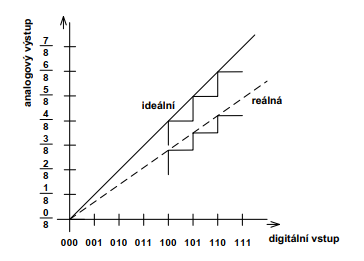
\includegraphics[scale=0.6]{images/CHzes.png}
   \end{center}
   \caption{Chyba zesílení}
\end{figure}

\textbf{Chyba nastavení nuly (offset)} - posunutí ideální převodní
charakteristiky o stejnou hodnotu
\begin{figure}[h]
   \begin{center}
     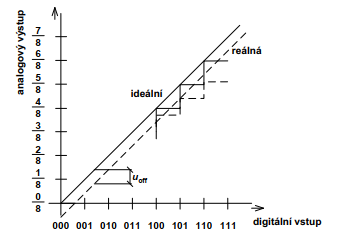
\includegraphics[scale=0.6]{images/offset.png}
   \end{center}
   \caption{Offset}
\end{figure}

\textbf{Chyba linearity (INL, DNL)} - nelinearita v globálu (INL) je
maximální vertikální rozdíl mezi ideální a reálnou převodní
charakteristikou.
\begin{figure}[h]
   \begin{center}
     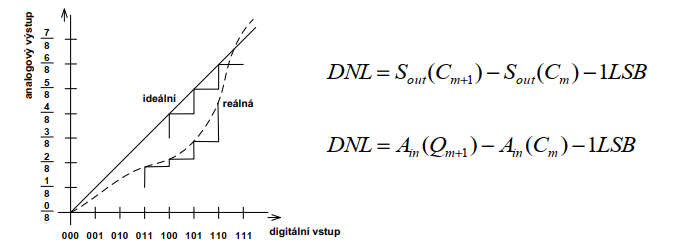
\includegraphics[scale=0.6]{images/CHlin.png}
   \end{center}
   \caption{Chyba linearity}
\end{figure}

Pokud by převodní charakteristika neměla monotónní růst nebo, pokles při růstu digitálního vstupu, pak je takový převodník
\textbf{nemonotónní}. Tato chyba je obvykle způsobena nesprávným odporem váhových rezistorů nebo nepřesným nastavením váhových zdrojů proudu. Platí, že pokud je DNL > 1LSB, pak je převodník nemonotónní.

\textbf{Kvantovací chyba} - způsobena konečným počtem diskrétních úrovní výstupního napětí a může dosahovat maximálně ± 1/2 hodnoty LSB.

\textbf{Hystereze} - způsobena nestejným průběhem převodní charakteristiky při změně tendence nastavovaných hodnot.
Zpravidla to způsobuje dielektrická absorbce kapacitorů. Absolutní chyba této odchylky závisí na rychlosti změny. Platí
tedy, že při dostatečně dlouhých intervalech mezi hodnotami se blíží tato chyba nule.

\textbf{Přípustné rozmezí výstupního napětí} - maximální výstupní napětí DAC s proudovým výstupem, při němž jsou ještě
garantovány všechny parametry převodníku.

\textbf{Průnik signálu} - nežádoucí pronikání signálu přes rozpojené spínače nebo části obvodu, které mají izolovat.


\subsubsection{Dynamické parametry}
Dynamické vlastnosti jsou také určeny dobou převodu T\textsubscript{P}, což je maximální doba potřebná k ustálení výstupní analogové veličiny na správnou hodnotu s povolenou chybou za předpokladu konstantní hodnoty digitálního signálu během převodu.

\textbf{Odstup signál-šum (SNR)} se vyhodnocuje z kmitočtového spektra signálu, kdy signál odpovídá základní harmonické. SNR závisí na počtu kvantovacích úrovní. Pro sinusový signál teoreticky platí:
\begin{equation}
SNR=(6,02*N+1,76)
\end{equation}

\textbf{Efektivní počet bitů} se určuje ze SNR:
\begin{equation}
N=\frac{SNR-1,76}{6,02}
\end{equation}

\textbf{Harmonické zkreslení (THD)} se zjišťuje při buzení DAC daty, která odpovídají digitalizovanému průběhu ideální sinusovky. Zkreslení je pak určeno z výstupního signálu
\begin{equation}
THD=20*log\frac{1}{2}*\frac{\sqrt{U_{2}^2+...+U_{N}^2}}{U_{1}}
\end{equation}

\textbf{SFDR} je parametr, který je důležitý zejména v případě, kdy má převodník vysoké převzorkování nebo je vyžadována
spektrální „čistota“ převodníku. SFDR je tedy určeno jako poměr mezi amplitudou užitečného signálu a největší složkou zkreslení.

\begin{figure}[h]
   \begin{center}
     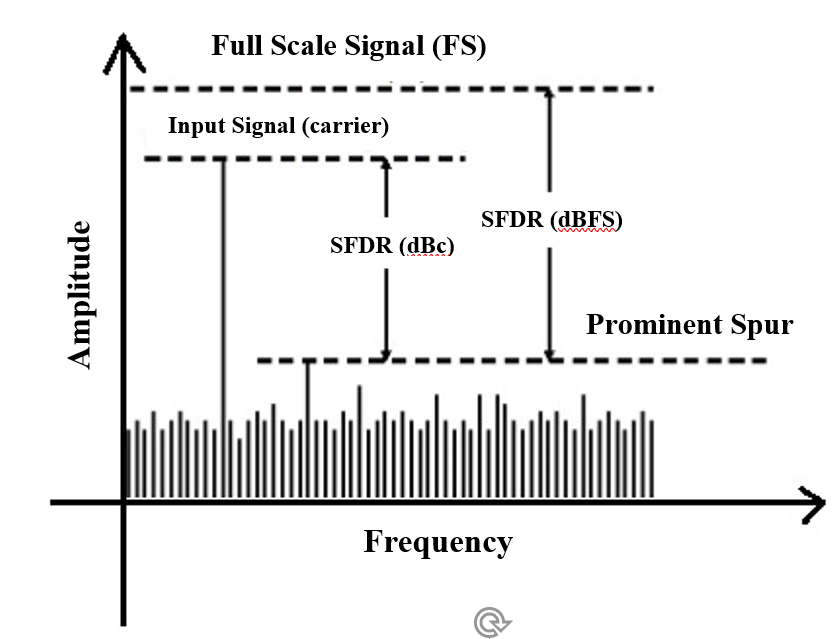
\includegraphics[scale=0.5]{images/Dyn.png}
   \end{center}
   \caption{Dynamické parametry}
\end{figure}

\textbf{Maximální rychlost převodu (správně četnost převodu)} - určena počtem vstupních slov D, která mohou být
převodníkem převedena na analogovou výstupní veličinu za jednotku času.

\textbf{Přechod výstupního analogového napětí} z jedné úrovně na jinou může být doprovázen přechodným dějem. Jestliže se neuvažují případné překmity zesilovače, je přechodný jev způsoben konečnou dobou sepnutí, resp. rozepnutí elektronických spínačů uvnitř struktury převodníku.


Přechody výstupního napětí mezi hladinami jsou provázeny \textbf{krátkými přechodovými špičkami (glitches)} -
výška může mnohonásobně přesáhnout hodnotu uLSB. Tato situace nastává při přepínání více spínačů, největší jsou při přechodu např. 01111111 → 10000000, kdy je nestejná rychlost sepnutí a rozepnutí spínačů. Tyto zákmity se odstraňují pomocí tzv. deglitcheru, což v praxi bývá rychlý vzorkovací obvod.
\begin{figure}[h]
   \begin{center}
     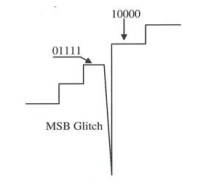
\includegraphics[scale=0.6]{images/Glitch.png}
   \end{center}
   \caption{Glitch}
\end{figure}

\subsection{Základní zapojení a funkce}
Paralelní převodníky DAC patří mezi nejrozšířenější typy, velmi často se vyrábějí monoliticky. Základní paralelní převodník čísla na proud a jeho činnost přímo odpovídá:
\begin{equation}
i = I*D=T*\frac{C}{2^n}
\end{equation}

kde I označuje referenční proud převodníkem. Převodník obsahuje celkem n řízených zdrojů konstantních proudů, které jsou ovládány logickými signály

\begin{figure}[h]
   \begin{center}
     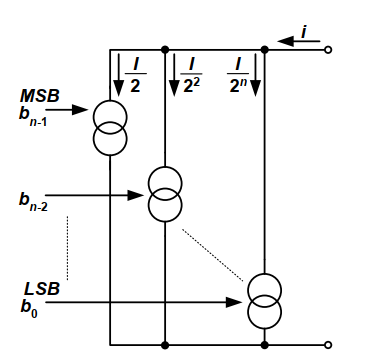
\includegraphics[scale=0.6]{images/DAzaklad.png}
   \end{center}
   \caption{Základní zapojení paralelního převodníku čísla na proud}
\end{figure}

Z principiálního zapojení je zřejmá hlavní nevýhoda a tou jsou vysoké požadavky na přesnost proudových zdrojů. Aby bylo dosaženo potřebné přesnosti převodu, musí proudové zdroje v jednotlivých větvích dodávat do obvodu přesně definovanou hodnotu váhového proudu a to i v přesném poměru vůči ostatním zdrojům. Jak je uvedeno v dalších kapitolách, lze tento nedostatek eliminovat zapojením společně s odporovou sítí R-2R.

\begin{figure}[h]
   \begin{center}
     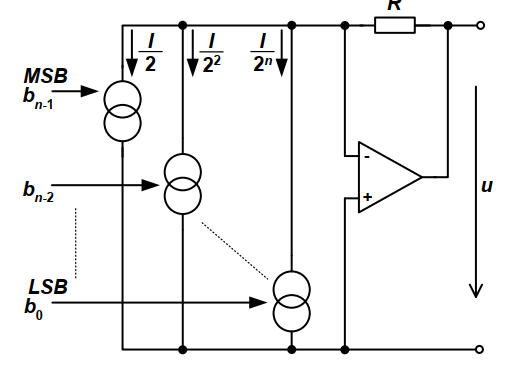
\includegraphics[scale=0.6]{images/DAU.png}
   \end{center}
   \caption{Paralelní převodník s napěťovým výstupem}
\end{figure}

Paralelní převodník s napěťovým výstupem může být jednoduše sestaven z předchozího převodníku D/I, který je doplněn o převodník I/U. Pro výstupní napětí platí:
\begin{equation}
u=i*R=R*\frac{I}{2^n}*\sum_{n-1}^{k=0}b_{k}2^k
\end{equation}


\section{Využití sítě R-2R a modifikace}
Výstup rezistorové sítě bývá nejčastěji připojen k převodníku I/U s OZ a výstupní veličinou je pak napětí. Rezistorové sítě se upravují zařazením sériových rezistorů do některých míst sítě. Tyto kombinované váhové sítě jsou tvořeny sekcemi váhových rezistorů opět spínaných řízenými spínači na zem nebo referenční napětí. 
































